\documentclass{article}
\usepackage{graphicx} % Required for inserting images
\usepackage[utf8]{inputenc}
\usepackage{amsmath}
\usepackage{asymptote}
\title{Central Limit Theorem}
\author{Hongning Wang}
\date{November 2023}

\begin{document}

\maketitle

In a sealed room, the instantaneous velocity of a single oxygen molecule is hard to predict at best. However, when one puts $16$ grams of oxygen (over $10^{26}$ molecules) in that same room, the average velocity forms a nice, normal distribution: the Boltzmann-Maxwell distribution. In fact, this distribution is so predictable that a close  variant (distribution of the magnitude of velocity) shows up in high school physics and chemistry exams.

So how did we get from a motion that was essentially random to a well-behaved motion? The answer is the central limit theorem, which basically says that in many cases the combination of many independent, identical variables, forms a normal distribution. This theorem works in all cases where each random variable is evenly distributed (gas molecules, dice rolls, coin flips, etc.).

First, we need some statistics background. For a random variable $X$, we define its probability density function $f(x) := \text{probability that } X = x$. For instance, $f(1) = \frac{1}{6}$ for a fair dice. Note particularly that the net area under the density curve is $1$. Additionally, any list of numbers has a mean $\mu$ and a standard deviation (average distance away from the mean) $\sigma$. A special case of the probability distribution is the normal distribution, which is defined as the function
\[ f(x) = \frac{1}{\sigma \sqrt{2\pi}} \cdot e^{-\frac{(x - \mu)^2}{2\sigma^2}}. \]

% if someone can insert the function below that would be awesome
\begin{center}
    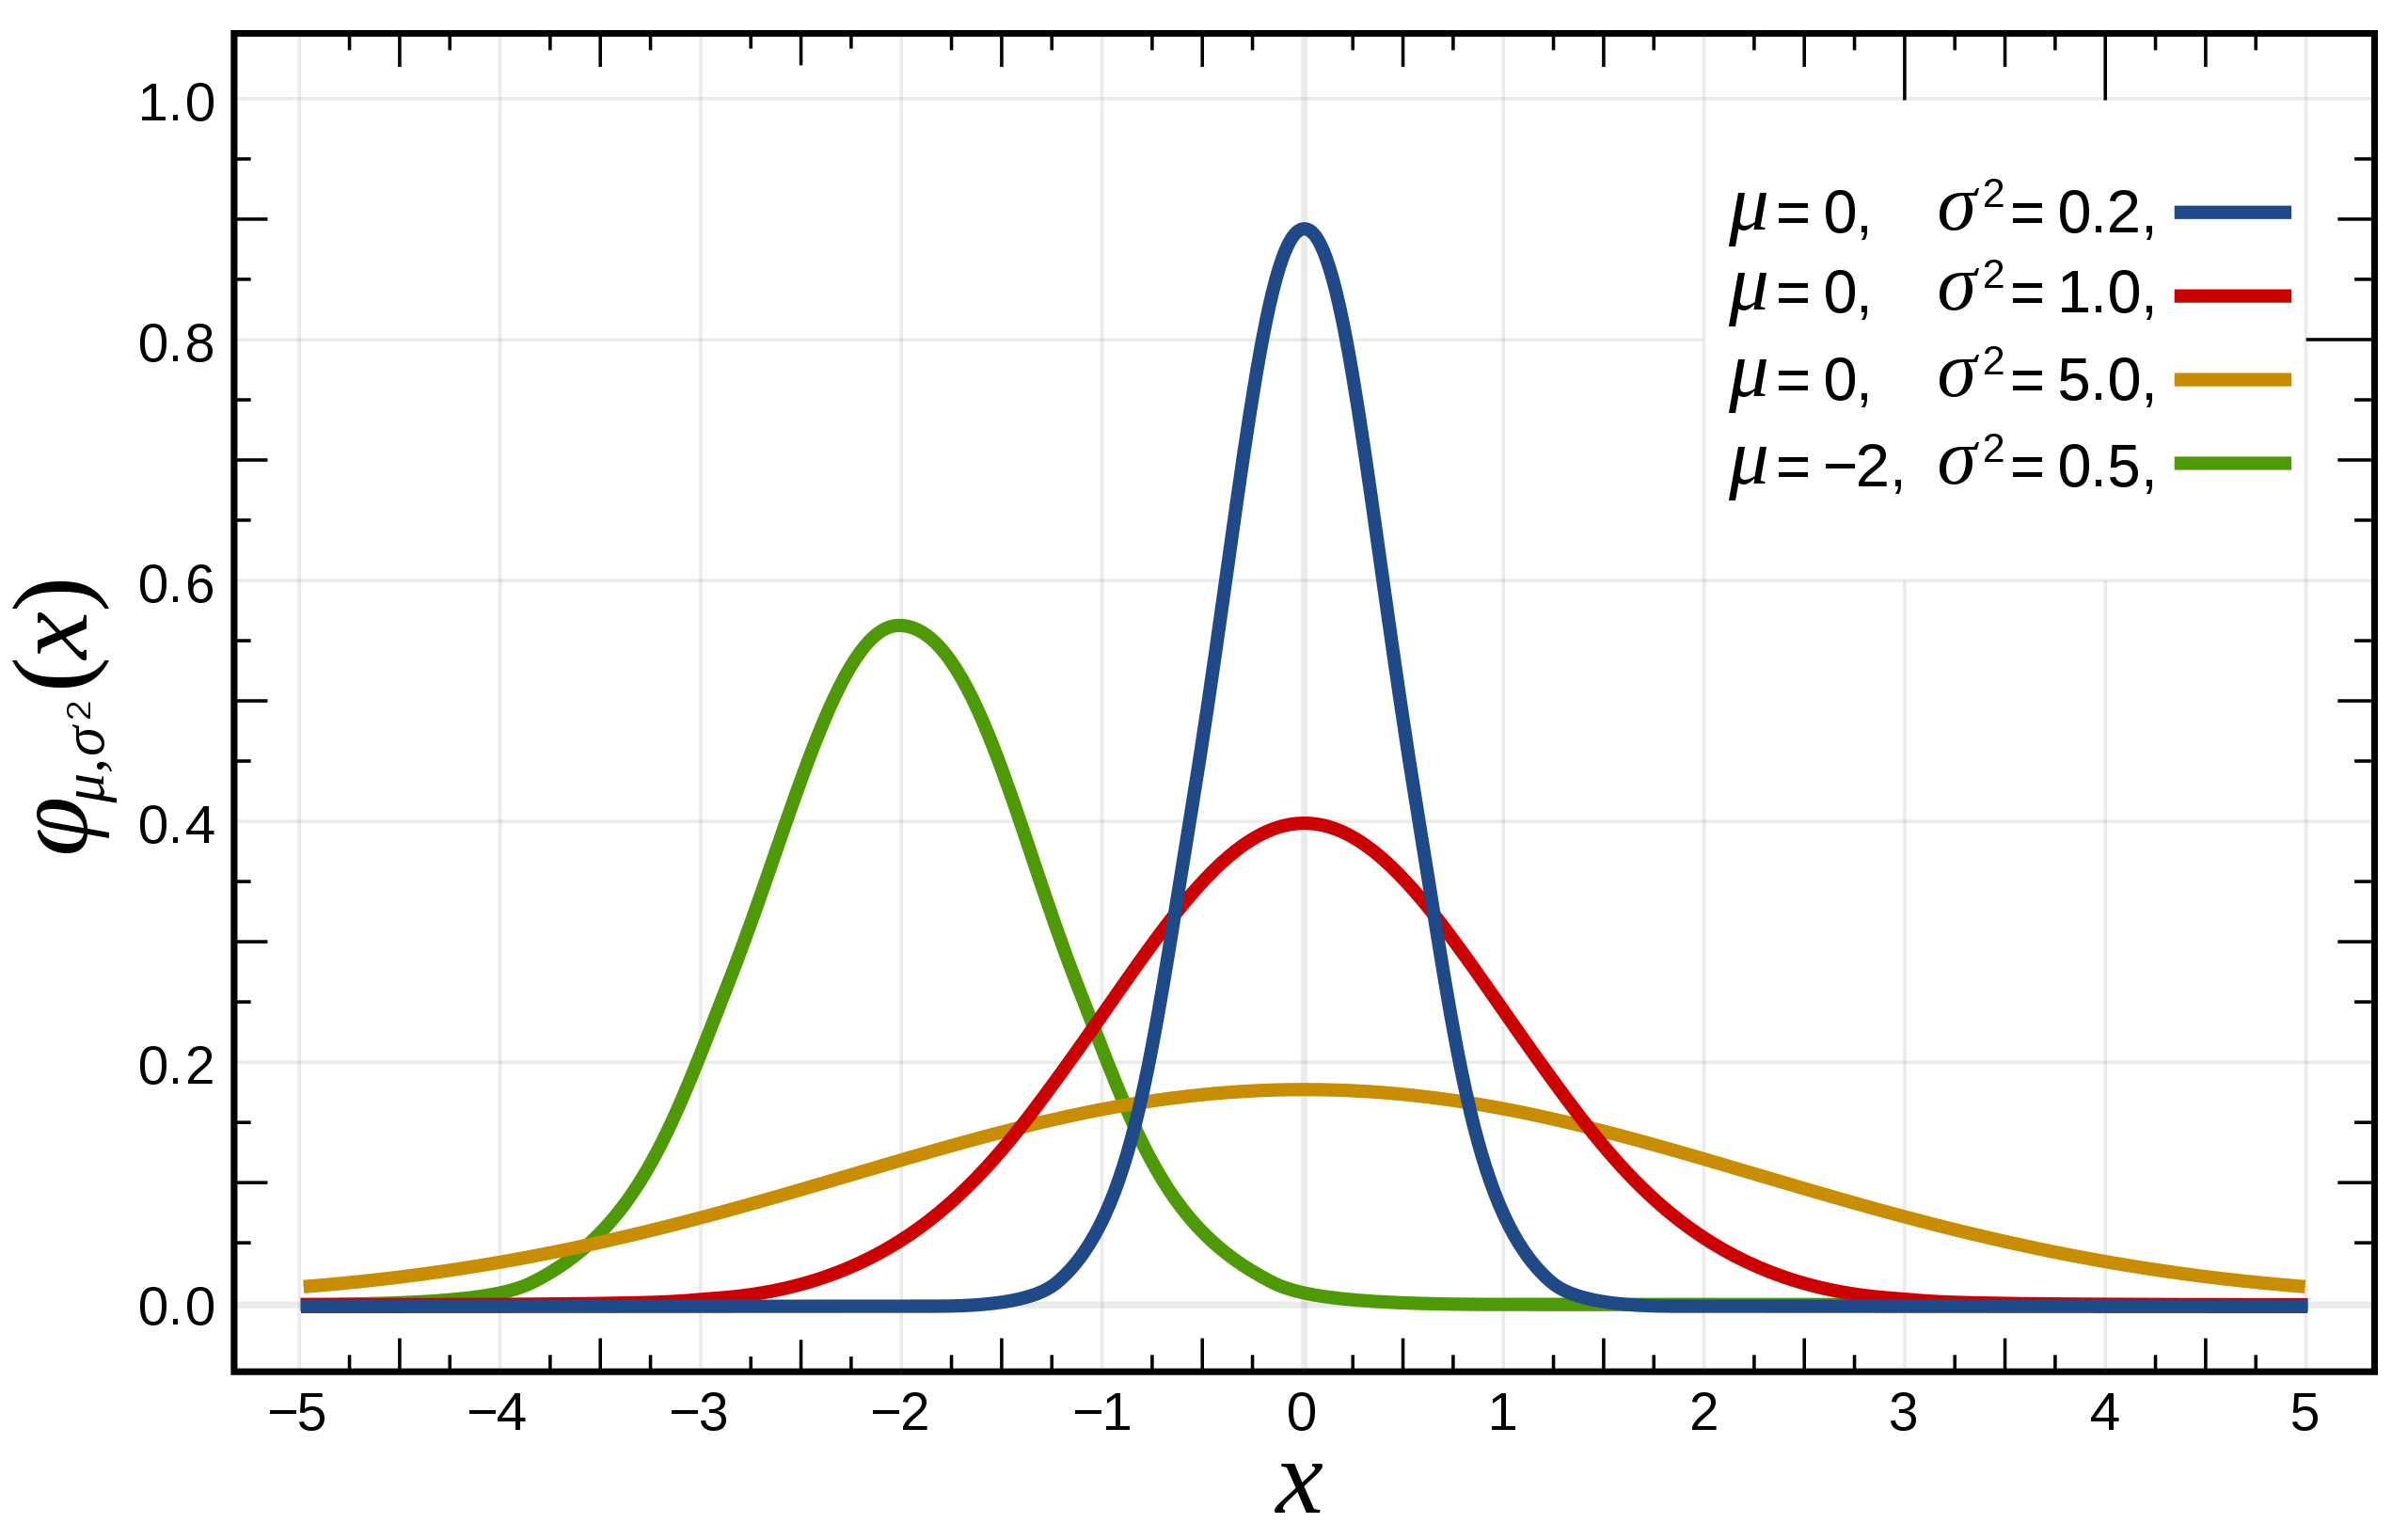
\includegraphics[width=5in, scale=0.1]{images/normal_distrib.png}
\end{center}
% CITE

This function is particularly nice because it is extremely common (due to the central limit theorem), peaks at the population mean, and behaves in well-documented ways at integer standard deviations away from the mean. 

Now, we return to the guiding question: how do a bunch of independent variables combine to form a normal distribution?

The fundamental idea is ubiquitous in probability: for two random variables $X$ and $Y$,
\[ P(X+Y=k) = \sum_{\text{all } x+ y = k} P(X=x)P(Y=y). \]
For example, the sum that the rolls from two dice sum to $3$ is the sum of the probability that the first dice is $1$ and the second is $2$ and the probability that the first is $2$ and the second is $1$. Now, when combining the density functions of two variables, there are more terms on the $RHS$ when $k$ is closer to the mean of the resulting sum. For instance, the probability of the sum of the rolls of two dice being $7$ (the mean) is $\frac{1}{6}$ while the probability of the sum being $2$ is $\frac{1}{36}$. Therefore, the convolution of many random variables produces a distribution that peaks around the mean of the variables' sum and declines away from the mean, as in the normal distribution. The actual math is quite complicated, and is beyond the scope of this article. 

Let us demonstrate the power of the theorem in the context of coin flips. Specifically, suppose I wanted to find the probability that I flipped between $780$ and $800$ heads when I flip $1600$ fair coins at once. First, the mean of the distribution of the number of heads is evidently $1600/2 = 800$ by symmetry. I'll also take a page from statistics and say that
\[ \sigma = \sqrt{n(p)(1-p)} = \sqrt{1600 \cdot 1/2 \cdot 1/2} = 20. \]
As a result, we are essentially finding the probability that the number of head flips is between $1$ and $0$ standard deviations away from the mean. This is well-known to be $34$\%, and can be easily calculated using normalcdf on a TI-calculator. 

Indeed, the real answer, which is much harder to calculate, is
\[ \sum_{n=780}^{800} \frac{\binom{1600}{n}}{2^{1600}} \]
and comes out to about $35.7$\%, which is remarkably close to our heuristic answer.

The central limit theorem plays a major role in the distribution of heights, birth weight, standardized test score, and more.

The other interesting way to look at the central limit theorem is that a large enough sample decently approximates the whole population. As such, the central limit theorem makes observational studies and experiments worthwhile. 


\end{document}
